%---------------------------------------------------------------------
\section{Resultados das simula��es}

%Simula��o utilizando \HI{\texttt{Matlab/Simulink}}.

%\subsection{Gradiente Normalizado}

Nas simula��es, procuramos avaliar o comportamento do sistema para as seguintes condi��es:
%
\begin{enumerate*}[label=(\roman*)]
\item condi��es iniciais $\theta(0)$ e $y(0)$;
\item Par�metros da planta e do modelo;
\item ganho de adapta��o $\Gamma$.
\end{enumerate*}

Apresentaremos os resultados obtidos atrav�s de simula��es no ambiente \HI{\texttt{Matlab/Simulink}} e os discutiremos na pr�xima se��o.

\subsection{Simula��o \#1}

Inicialmente, desejamos verificar o comportamento do sistema para varia��es nas
condi��es iniciais.

\bigskip

\textbf{\underline{Simula��o 1.1}: sistema de 2$^\text{a}$ ordem}
%
\begin{align*}
  y &= \frac{s+1}{s^2+4s+4}u\,,  &  \Lambda &= s+1\,, & \HI{\theta(0) &=
  \mathbf{0}, \mathbf{1}}\,, \\
  \gamma &= 10 \, \textbf{I}_4\,, & r &= 10\textrm{0.63sin}(t) +
  25\textrm{4.5sin}(t) \,.
\end{align*}

\begin{figure}[H]
  \centering
  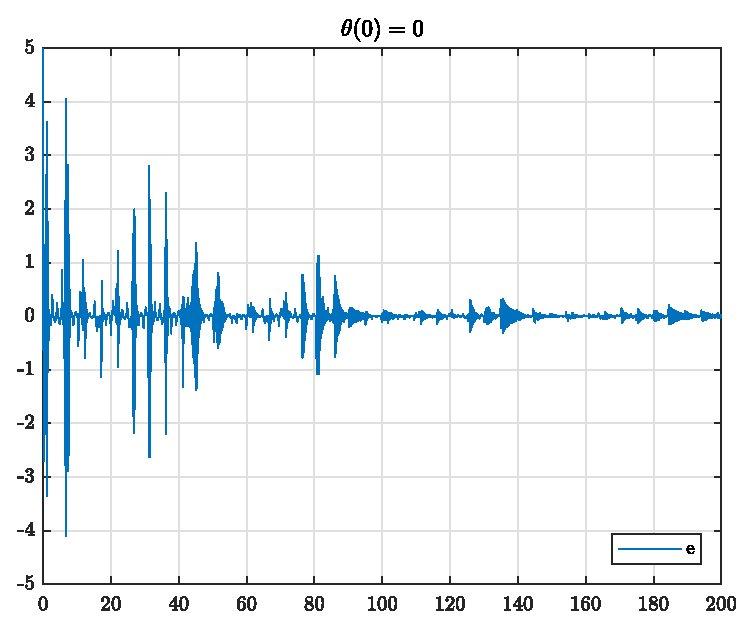
\includegraphics[width=12cm]{figs/en2t0.eps} 
\end{figure}

\begin{figure}[H]
  \centering
  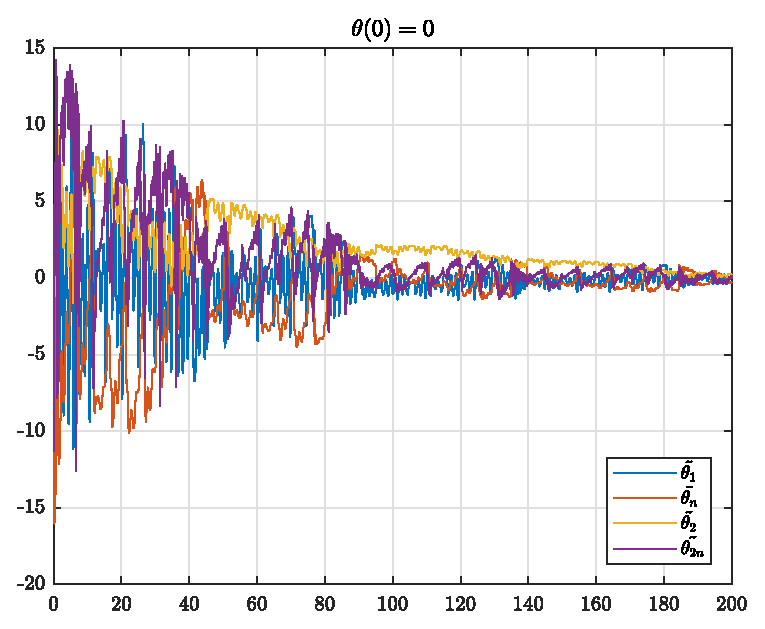
\includegraphics[width=12cm]{figs/tiln2t0.eps} 
\end{figure}